\documentclass[conference]{IEEEtran}
\thispagestyle{plain} % remove for final version
%\IEEEoverridecommandlockouts
% The preceding line is only needed to identify funding in the first footnote. If that is unneeded, please comment it out.
\usepackage{cite}
\usepackage{amsmath,amssymb,amsfonts}
\usepackage{algorithmic}
\usepackage{graphicx}
\usepackage{textcomp}
\usepackage{listings}
\usepackage{amsmath}
\usepackage{multirow}
\usepackage{enumitem}
\usepackage{hyperref}
\newcommand\recheck[1]{\textcolor{red}{#1}}
\def\BibTeX{{\rm B\kern-.05em{\sc i\kern-.025em b}\kern-.08em
    T\kern-.1667em\lower.7ex\hbox{E}\kern-.125emX}}

% Very convenient to add comments on the paper. Just set the boolean
% to false before sending the paper:
\usepackage{ifthen}
\usepackage{balance}
\newboolean{showcomments}
\setboolean{showcomments}{true}
%\setboolean{showcomments}{false}
\ifthenelse{\boolean{showcomments}}
{ \newcommand{\mynote}[2]{\textcolor{red}{
    \fbox{\bfseries\sffamily\scriptsize#1}
    {\small$\blacktriangleright$\textsf{\emph{#2}}$\blacktriangleleft$}}}}
{ \newcommand{\mynote}[2]{}}

\newcommand{\jl}[1]{\mynote{Julia}{#1}}
\newcommand{\jh}[1]{\mynote{Comments}{#1}}
\newcommand{\ro}[1]{\mynote{Richard}{#1}}
\newcommand{\jg}[1]{\mynote{James}{#1}}
\newcommand{\ty}[1]{\mynote{Yuan}{#1}}
\newcommand{\ans}[1]{{#1}}

\usepackage[dvipsnames]{xcolor}
  \definecolor{diffstart}{named}{Blue}%{Grey}
  \definecolor{diffincl}{named}{OliveGreen}
  \definecolor{diffrem}{named}{Red}

\newcommand{\extrabold}{\bfseries}

\lstset{numbers=left,xleftmargin=3em}

\usepackage{listings}
  \lstdefinelanguage{diff}{
	basicstyle=\ttfamily\extrabold\tiny,
	morecomment=[f][\color{diffstart}]{@},
	morecomment=[f][\color{diffincl}]{+},
	morecomment=[f][\color{diffrem}]{-},
        numbers=left,
        stepnumber=1,
        keepspaces=true,
	identifierstyle=\color{black},
  }


\thispagestyle{plain} % remove for final version
\pagestyle{plain} % remove for final version

\usepackage{pgfplots}
\pgfplotsset{width=3in,height=1.5in,compat=1.14}

\begin{document}



% \title{Hierarchical Learning of Patch Embedding for Stable Patch Identification in Linux Kernel}
% \title{PatchNet: Hierarchical Deep Learning-Based Stable Patch Identification for the Linux Kernel}
\title{PatchNet: A Tool  for Deep Patch Classification}
% {\footnotesize \textsuperscript{*}Note: Sub-titles are not captured in Xplore and
% should not be used}
% \thanks{Identify applicable funding agency here. If none, delete this.}
% }
%
% \author{\IEEEauthorblockN{Thong Hoang\textsuperscript{1}, Julia Lawall\textsuperscript{2}, Richard J. Oentaryo\textsuperscript{3}, Yuan Tian\textsuperscript{1}, David Lo\textsuperscript{1}}
% \IEEEauthorblockA{\textsuperscript{1}School of Information Systems, Singapore Management University, Singapore\\
% \textsuperscript{2}Inria/LIP6, Regal\\
% \textsuperscript{3}McLaren Applied Technologies, Singapore}
% vdthoang.2016@smu.edu.sg, julia.lawall@lip6.fr, richard.oentaryo@mclaren.com, \{ytian, davidlo\}@smu.edu.sg
% }

\maketitle

\begin{abstract}
% This document is a model and instructions for \LaTeX.
% This and the IEEEtran.cls file define the components of your paper [title, text, heads, etc.]. *CRITICAL: Do Not Use Symbols, Special Characters, Footnotes, 
% or Math in Paper Title or Abstract.

%Linux kernel stable versions serve the needs of users who value stability
%of the kernel over new features. The quality of such stable kernel versions
%depends on the initiative of kernel maintainers to propagate bug fixing
%patches to the stable versions. Thus, it is desirable to consider to what
%extent this process can be automated. A previous approach
%% based on Learning from Positive and Unlabeled Examples (SVM) and Support Vector Machine (SVM) 
%relies on words from commit messages and a small set of manually constructed code
%features. This approach, however, shows only moderate accuracy.
%In this paper, we investigate whether deep learning can provide a more
%accurate solution. We propose PatchNet, a hierarchical deep learning-based approach that is capable of automatically extracting features from commit messages and commit code and using them to identify stable patches. PatchNet contains a deep hierarchical structure that mirrors the hierarchical and sequential structure of commit code, making it distinctive from the existing deep learning models on source code.
%% \ty{I add this sentence highlighting the novelty of PatchNet. James,pls verify this.} 
%Experiments on 82,403 recent Linux patches confirm the superiority of   
%PatchNet against various state-of-the-art baselines, including the one actively-used by Linux kernel maintainers. 
% The results show that PatchNet surpasses the best-performing baseline by 6.55\%, 7.8\%, and 6.3\% in terms of accuracy, F1, and AUC, respectively. 
% 6.55\%, 0.12\%, 16.13\%, 7.8\%, and 6.3\%,\ty{not consistent with the ones reported in experiment section} in terms of accuracy, precision, recall, F1, and AUC, respectively. 

% Linux kernel stable versions serve the needs of users who value stability of the kernel over new features. The quality of such stable kernel versions depends on the initiative of kernel maintainers to propagate bug fixing patches to the stable versions. Thus, it is desirable to consider to what extent this process can be automated. In this work, we propose PatchNet, an automated tool based on a hierarchical deep learning-based approach to extract features from commit messages and commit code and using them to identify stable patches. PatchNet contains a deep hierarchical structure that mirrors the hierarchical and sequential structure of commit code, making it distinctive from the existing deep learning models on the source code. PatchNet accepts as input a set of patches to train a predicted model. We then apply the predicted model on a new set of patches to collect a list of predicted scores of given patches used to estimate how likely the given patches are bug fixing patches. Noticeably, our implementation of PatchNet provides several options allowing users to select parameters for the training process. Moreover, our tool is applicable to 

Identifying bug fixing patches is an important problem as it serves the needs of users who want to take advantages of the latest features. Thus, it is desirable to consider to what extent this process can be automated. However, writing an application used to solve this problem is time-consuming and requires skills from developers. In this work, we propose PatchNet, an automated tool based on a hierarchical deep learning-based approach to extract features from commit messages and commit code and using them to identify stable patches. PatchNet contains a deep hierarchical structure that mirrors the hierarchical and sequential structure of commit code, making it distinctive from the existing deep learning models on the source code. PatchNet accepts as input a set of patches to train a predicted model. We then apply the predicted model on a new set of patches to collect a list of predicted scores of given patches used to estimate how likely the given patches are bug fixing patches. Noticeably, our implementation of PatchNet provides several options allowing users to select parameters for the training process. Moreover, the tool is also applicable to other problems in software engineering domains such as defect prediction, bug localization, etc. 
\end{abstract}


%\begin{IEEEkeywords}
%Linux kernel, bug fixing, classification, deep learning.
%\end{IEEEkeywords}

\vspace{-0.25cm}
\section{Introduction}
\label{sec:intro}

Deep learning techniques have been widely used to solve many problems in software engineering such as code clone detection~\cite{white2016deep,li2017cclearner}, software traceability link recovery~\cite{guo2017semantically}, bug localization~\cite{huo2016learning, lam2017bug}, defection prediction~\cite{yang2015deep, wang2016automatically}, etc. However, these techniques have not been applied to learn a semantic representation of patches for similar tasks such as patch identification, patch classification, etc. 

These tasks are popular in the Linux kernel as the Linux kernel requires that all patches applied to a stable version need to pass through a mainline first. A mainline subsystem \textit{maintainer} may identify a patch as a bug fixing patch appropriate for stable kernels. Stable-kernel maintainers then apply the resulting patches to the stable version that are affected by the bug. The quality of the stable kernels critically relies on the effort that the subsystem maintainers put into labeling patches as relevant to the stable kernels, i.e., identifying \textit{stable patches}. This manual
effort represents a potential weak point in the development process, e.g., the maintainers may forget to label some relevant patches, and different maintainers could apply different criteria for selecting them.

To address the above problem, Tian et al.~\cite{tian2012identifying} presented an approach that combines LPU (Learning from Positive and Unlabeled Examples)~\cite{letouzey2000learning} and SVM (Support Vector Machine)~\cite{suykens1999least} to automatically identify bug fixing patches for Linux stable kernels. The LPU+SVM based approach relies on thousands of bag-of-words\footnote{A bag-of-words model represents a text as the multi-set of the words it contains.} features extracted from commit messages and 52 manually features extracted from code changes. However, the bag-of-words representation of commit message implies that the temporal dependencies (ordering) of words in a commit message are ignored. In addition, the manual creation of code features might overlook features that maintainers find helpful to identify stable patches. Thus, a richer feature representation of a patch that captures its hierarchical and structural properties is needed.

In this work, we implement a prototype tool based on our new work, submitted to ICSE'19, that performs deep learning on a set of patches. We name the tool PatchNet which is a tool for deep patch classification. The tool takes as input a set of patches and outputs a list of predicted scores used to estimate how likely the given patches the given patches are bug fixing patches. Specifically, PatchNet aims to automatically learn two embedding vectors for representing the commit message and the set of code changes in a given patch, respectively. The two embedding vectors are then used to compute a prediction score of a given patch to estimate how likely the given patch is bug fixing patch.

Moreover, PatchNet is applicable to other problems in the software engineering domain such as bug localization, defect prediction, etc. For example, bug localization often contains bug reports and source code files. The IR-based bug localization techniques~\cite{rao2011retrieval, sisman2012incorporating} analyze textual descriptions contained in bug reports and identifier names and comments in source code files. They then return a ranked list of program elements (typically program files) that are the most similar to the bug reports. In order to solve this problem in PatchNet, we can input bug reports and source code files as commit messages and commit code, we then train PatchNet model and output predicted scores measuring how likely the given source files relevant to the bug reports. 

The rest of this paper is organized as
follows. Section~\ref{sec:design} highlights the bird's-eye view architecture of PatchNet. Section~\ref{sec:usage} illustrate how PatchNet works with specific examples as well as demonstrates command line options. Section \ref{sec:related_work} discuss related works. Finally, we conclude and present future work in  Section~\ref{sec:conclusion}.

%Different from existing deep learning techniques working on source code~\cite{white2016deep,huo2017enhancing,wang2016automatically,lam2017bug}, we propose a
% novel hierarchical representation learning architecture for patches, by constructing embedding vectors of a given patch in a bottom-up fashion. PatchNet first constructs embedding vectors of removed code and added code of an affected file in the given patch. The embedding vectors are able to capture the sequential nature of the removed and added code. These are then concatenated to build an embedding vector for the affected file. In turn, the embedding vectors of all the affected files are used to build the representation of the entire code changes in the given patch.





% The word features are obtained automatically by representing each commit message as a bag of words,\footnote{A bag-of-words model represents a text as the multi-set of the words it contains.} whereas the code features are defined manually. However, the bag-of-words representation of commit message implies that the temporal dependencies (ordering) of words in a commit message are ignored. In addition, the manual creation of code features might overlook features that maintainers find helpful to identify stable patches. Thus, a richer feature representation of a patch that captures its hierarchical and structural properties is needed.

% The Linux kernel follows a two-tiered release model in which a \textit{mainline} version, accepting bug fixes and feature enhancements, is paralleled by a series of stable versions that accept only bug fixes~\cite{lee2003firm}. 
% The mainline serves the needs of users who want to take advantage of the latest features, while the stable versions serve the needs of users who value stability, or cannot upgrade their kernel due to hardware and software dependencies. To ensure that there is as much review as possible of the bug fixing patches and to ensure the highest quality of the mainline itself, the Linux kernel
% requires that all patches applied to the stable versions pass through the mainline first. A mainline subsystem \textit{maintainer} may identify a patch as a bug fixing patch
% appropriate for stable kernels and add to the commit log a Cc: stable tag.\footnote{The exact tag is \textrm{Cc}: \textrm{stable@vger.kernel.org}.} Stable-kernel maintainers then extract such annotated commits from the mainline commit history and apply the resulting patches to the stable versions that are affected by the bug.

% Figure~\ref{fig:sample_patch} shows a sample bug fixing patch that has been applied to
% the stable version derived from Linux v4.5. This patch adjusts a returned
% error code that may influence the value reported to the user level. As
% illustrated in Figure~\ref{fig:sample_patch}, a patch contains both a
% textual commit message (lines 5-12) and a set of diff code elements (lines
% 14-28), i.e., changes that are applied to the affected file. A patch
% \textit{author} submits a patch to \textit{maintainers}. The
% maintainers decide whether the patch should be integrated into the
% mainline kernel, and if so, whether it should be annotated for propagation
% to stable kernels.

% \begin{figure}[t!]
% \begin{lstlisting}[language=diff]
% commit 342da5cefddbf818e1cb59537e021cdad9744e93
% Author: Alex Lyakas <...>
% Date:   Thu Mar 10 13:09:46 2016 +0200

%     btrfs: csum_tree_block: return proper errno value
    
%     commit 8bd98f0e6bf792e8fa7c3fed709321ad42ba8d2e upstream.
    
%     Signed-off-by: Alex Lyakas <...>
%     Reviewed-by: Filipe Manana <...>
%     Signed-off-by: David Sterba <...>
%     Signed-off-by: Greg Kroah-Hartman <...>

% diff --git a/fs/btrfs/disk-io.c b/fs/btrfs/disk-io.c
% index d8d68af..87946c6 100644
% --- a/fs/btrfs/disk-io.c
% +++ b/fs/btrfs/disk-io.c
% @@ -303,7 +303,7 @@ static int csum_tree_block(struct btrfs_fs_info *fs_info,
%                 err = map_private_extent_buffer(buf, offset, 32,
%                                         &kaddr, &map_start, &map_len);
%                 if (err)
% -                       return 1;
% +                       return err;
%                 cur_len = min(len, map_len - (offset - map_start));
%                 crc = btrfs_csum_data(kaddr + offset - map_start,
%                                       crc, cur_len);
% @@ -313,7 +313,7 @@ static int csum_tree_block(struct btrfs_fs_info *fs_info,
% ...
% \end{lstlisting}\vspace{-0.4cm}
% \caption{A sample bug fixing patch in Linux kernel v4.5.}
% \label{fig:sample_patch}\vspace{-0.4cm}
% \end{figure}

% The quality of the stable kernels critically relies on the effort that the
% subsystem maintainers put into labeling patches as relevant to the
% stable kernels, i.e., identifying \textit{stable patches}. This manual
% effort represents a potential weak point in the development process, e.g., the maintainers may forget to label some relevant patches, and
% different maintainers could apply different criteria for
% selecting them. While the stable-kernel maintainers can themselves
% additionally pick up relevant patches from the mainline commits, there are
% hundreds of such commits per day, making it likely that many will slip
% past~\cite{lee2003firm}. This task can thus benefit from automated assistance.
% \jg{David suggestion: Could we get a quote from Linux kernel maintainers on the need for such system? This can better motivate the problem.}

% \jg{TY: Can you please recheck the paragraph below?}

% Tian et al.~\cite{tian2012identifying} presented an approach that
% combines LPU (Learning from Positive and Unlabeled
% Examples)~\cite{letouzey2000learning} and SVM (Support Vector
% Machine)~\cite{suykens1999least} to automatically identify bug fixing
% patches for stable versions. This LPU+SVM based approach relies on
% thousands of word features extracted from the commit messages and 55
% features extracted from code changes. The word features are obtained
% automatically by representing each commit message as a
% bag of words,\footnote{A bag-of-words model represents a text as the multi-set of
%   the words it contains.} whereas the code features are defined
% manually to characterize how likely a given patch is a bug fixing patch. We note that not all bug fixes are relevant 
% However, the bag-of-words 
% representation of the commit message implies that the temporal dependencies (ordering) of
% words in a commit message are
% ignored. 
% In addition, the manual creation of code features might overlook
% features that maintainers find helpful to
% identify bug fixing patches.
% Thus, a richer feature representation of a patch that captures its inherent
% and relevant properties by considering both its commit message and
% corresponding code changes is needed. 

% Tian et al.~\cite{tian2012identifying} presented an approach that combines LPU (Learning from Positive and Unlabeled Examples)~\cite{letouzey2000learning} and SVM (Support Vector Machine)~\cite{suykens1999least} to automatically identify bug fixing patches for Linux stable kernels. 
% % We note that not all bug fixes are relevant for stable kernels, there are some bugs having low impact or the fix is too complex to be considered, hence the problem of identifying bug fixing patches is close to that of identifying stable patches.\ty{need verification} 
% This LPU+SVM based approach relies on thousands of word features extracted from commit messages and 52 features extracted from code changes. The word features are obtained automatically by representing each commit message as a bag of words,\footnote{A bag-of-words model represents a text as the multi-set of the words it contains.} whereas the code features are defined manually. However, the bag-of-words representation of commit message implies that the temporal dependencies (ordering) of words in a commit message are ignored. In addition, the manual creation of code features might overlook features that maintainers find helpful to identify stable patches. Thus, a richer feature representation of a patch that captures its hierarchical and structural properties is needed.  
%by considering both its commit message and corresponding code changes is needed. 

%% \ty{we should
%% highlight our design that leveraging structural nature of the patch below,
%% it's not clear why such information is needed for identifying
%% stable-relevant patches.}

% To address the above problems, we propose PatchNet to automatically identify
% stable-relevant patches for the Linux kernel. Deviating from
% the previous LPU+SVM work, which requires human effort to construct code
% features, PatchNet aims to automatically learn two embedding vectors for
% representing the commit message and the set of code changes in a given
% patch, respectively. The two embedding vectors are then used to compute a
% prediction score of a given patch. The key challenge in achieving this
% goal is to accurately represent the structure of code changes, which are
% not contiguous text like the commit message, but rather amount to scattered
% fragments of removed and added code across multiple files. 
% Thus, different
% from existing deep learning techniques working on source
% code~\cite{white2016deep,huo2017enhancing,wang2016automatically,
% lam2017bug}, 
% we propose a
% novel hierarchical representation learning architecture for patches, named PatchNet, by constructing embedding vectors of a given patch in a bottom-up fashion. PatchNet first constructs embedding vectors of removed code and added code of an affected file in the given patch. The embedding vectors are able to capture the sequential nature of the removed and added code. These are then concatenated to build an embedding vector for the affected file. In turn, the embedding vectors of all the affected files are used to build the representation of the entire code changes in the given patch.

% we propose a novel hierarchical deep learning-based architecture for code changes by taking into account its structure, i.e., changes to different files, changes in different hunks, and changes in each code line (removed and added code). We also capture the sequential nature of source code by considering each line in commit code as a sequence of words. Our model first extracts embedding vectors of removed code and added code of
% an affected file in the given patch. These embedding vectors are then used to form the structure of code changes (i.e., hunks, lines) in the affected file. This structure then is used to build the representation of the code changes in the given commit.

% we propose a new representation learning architecture for code
% changes by constructing embedding vectors of removed code and added code of
% an affected file in the given patch. The embedding vectors are able to
% capture the sequential nature of the source code inside the code changes
% and are learned following a 3D convolutional neural network
% (3D-CNN) framework~\cite{ji20133d, maturana2015voxnet, su2015multi}. The embedding vectors are then
% concatenated to build an embedding vector for the affected file. In turn,
% the embedding vector of the file is used to build the representation of the
% code changes in the given commit.

% The main contributions of this paper include:

% \begin{itemize}[leftmargin=0.4cm]
% \item We take a closer look at the manual process of identifying patches for Linux stable versions and summarize the challenges faced by machine learning in automating this process.
% % \jg{David comment:To claim this contribution we need to do a non-trivial empirical study work and the findings must be well characterized. I wonder have we done that  ...  ? First contribution is typically the most important one. We need to be able to justify this one.}
  
%  \item In PatchNet, we propose a novel framework to construct an embedding vector for code changes inside a patch, based on both their sequential contents and hierarchical structure, while reusing a commonly employed deep learning strategy to
% process text data for representing the commit message.
 
%  %In PatchNet, we propose a novel framework to construct an embedding vector for code changes inside a patch, based on both their contents and structure.
%   %, while reusing a commonly employed deep learning strategy to process text data for representing the commit message.
% \item We evaluate our proposed approach on a new dataset that contains 82,403
%   recent Linux
%   patches. The experiments show the superiority of PatchNet compared to state-of-the-art baselines.  
% %   \ty{not consistent with the ones reported in the data collection section, please also verify the ones reported in the abstract}.
% \end{itemize}

%The rest of this paper is organized as
%follows. Section~\ref{sec:background} introduces background
%information. Section~\ref{sec:approach} elaborates the proposed PatchNet
%approach, followed by presentation of the experimental results in Section~\ref{sec:exp}. Section~\ref{sec:threat} discusses potential
%threats to validity, and Section \ref{sec:related_work} presents an overview of related work. Finally, Section~\ref{sec:conclusion} concludes and presents future work.

\section{Overall Design}
\label{sec:design}

\begin{figure}[!t]
	\center
	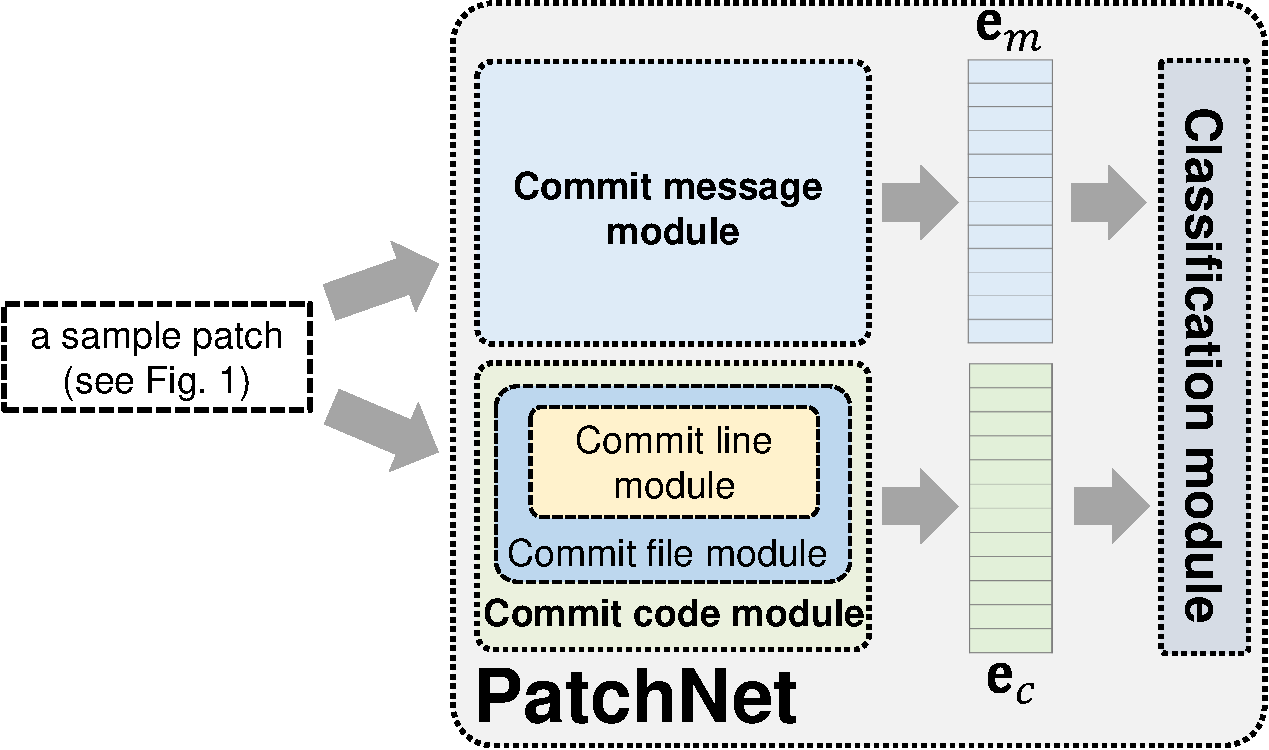
\includegraphics[scale=0.37]{figures/framework_overall_ver1.pdf}
	\caption{The proposed PatchNet framework. $\textbf{e}_m$ and $\textbf{e}_c$ are embedding vectors collected from the commit message module and commit code module respectively.}
	\label{fig:patchnet}
    \vspace{-0.4cm}
\end{figure}
\section{Usage Scenarios}
\label{sec:usage}
\section{Related Work}
\label{sec:related_work}

Researchers have applied deep learning techniques to solve software
engineering problems, including code clone
detection~\cite{white2016deep,li2017cclearner,bui2018hierarchical}, software traceability link
recovery~\cite{guo2017semantically}, bug
localization~\cite{huo2016learning, lam2017bug}, defect
detection~\cite{yang2015deep, wang2016automatically}, automated program
repair~\cite{gupta2017deepfix}, and API
learning~\cite{gu2016deep}. However, we did not find any work that applied
deep learning techniques to learn semantic representations of patches for
similar tasks such as stable patch identification, patch classification, etc. Here, we briefly describe the most closely related work besides the baseline approaches described in Section~\ref{sec:baselines}.


%\vspace{0.1cm} \noindent {\em Sequence-to-sequence learning.} Gu et al. adopted a neural language model named a Recursive Neural Network (RNN)~\cite{hagan1996neural, mikolov2010recurrent} encoder-decoder to generate API usage sequences, i.e., a sequence of method names, for a given natural language query~\cite{gu2016deep}. Gupta et al. proposed DeepFix to automatically fix syntax errors in C code~\cite{gupta2017deepfix}. DeepFix leverages a multi-layered sequence-to-sequence neural network with attention~\cite{mnih2014recurrent}, to process the input code and a decoder RNN with attention that generates the output fixed code. The above studies focus on learning sequence-to-sequence mappings and thus consider a different task than the one considered in our work.

%\vspace{0.1cm} \noindent {\em Learning code representation.}
CCLearner~\cite{li2017cclearner} learns a deep neural network classifier
from clone pairs and non clone pairs to detect clones.  To represent code,
it extracts features based on different categories (reserved words,
operators, etc.) of tokens in source code. White et al. presented another
deep learning based clone detector~\cite{white2016deep}. Their tool first
uses RNN to map program tokens to continuous-valued vectors, and then uses
RNN to combine the vectors with extracted syntactic features to train a
classifier. Wang et al. used a Deep Belief Network
(DBN)~\cite{hinton2009deep} to predict defective
code~\cite{wang2016automatically}. The DBN learns a semantic representation
(in the form of a continuous-valued vector) of each source code file from
token vectors extracted from programs' ASTs. Lam et al. combined deep
learning with information
retrieval to localize
buggy files based on bug reports~\cite{lam2017bug}. Bui and Jiang
proposed a deep learning based approach to automatically learn
cross-language representations for various kinds of structural code
elements (i.e., expressions, statements, and methods) for program
translation~\cite{bui2018hierarchical}. Different from the above
studies, we design a novel deep learning architecture that focuses on code
changes, taking into account their hierarchical and structural properties.

%Different from the above studies, we design a novel deep learning solution that: (1) learns representations of both text (in our case, commit logs) and code, and (2) considers code changes (i.e., diffs) rather than a source code file. 
%and (3) considers the hierarchical and sequential structure of code changes.


%\vspace{0.1cm} \noindent {\em Learning of both code and text representations.} Huo and Li proposed a model, LS-CNN, for classifying if a source code file is related to a bug report (i.e., the source code file needs to be fixed to resolve the bug report)~\cite{huo2017enhancing}. LS-CNN is the first code representation learning method that combines CNN and LSTM (a specific type of RNN) to extract semantic representations from \jl{from or of?} both code (in their case: a source code file) and text (in their case: a bug report). Similar to LS-CNN, PatchNet also learns semantic representations of \jl{from or of?} both code and text. However, different from LS-CNN, PatchNet includes a new representation learning architecture for commit code comprising the representations of removed code and added code of an affected file in a given patch. The representation of removed code and added code is able to capture the sequential nature of the source code inside a code change and it is learned following a CNN-3D architecture~\cite{ji20133d}, instead of LSTM. Our results in Section~\ref{sec:exp} show that PatchNet can achieve an 11.24\% improvement in terms of F1 over the LS-CNN model.

%\jl{The following seemed out of place in Section 3:}
%\jg{I'll ask Tian Yuan to take a look at this part.}
%Tian et al.~\cite{tian2012identifying} manually extracted code change features, i.e., number of files, number of hunks, etc., from a set of diff code changes, but that work does not break up the code changes by a file. Features extracted from code changes for each file may provide more information about the overall code changes by a given patch.

\vspace{-0.1cm}
\section{Conclusion}
\label{sec:conclusion}

In this paper, we propose PatchNet, a hierarchical deep learning-based model for identifying stable patches in the Linux kernel. For each patch, our model constructs embedding vectors from the commit message and the set of code changes. The embedding vectors are concatenated and then used to compute a prediction score for the patch. Different from existing deep learning techniques working on the source code~\cite{white2016deep, wang2016automatically, huo2017enhancing, li2017cclearner, guo2017semantically, lam2017bug, gu2016deep}, our hierarchical deep learning-based architecture takes into account the structure of code changes (i.e., files, hunks, lines) and the sequential nature of source code (by considering each line of code as a sequence of words) to predict stable patches in Linux kernel. 

% PatchNet learns a representation of code changes by constructing embedding vectors of removed and added code of an affected file in the given patch. We concatenate these embedding vectors to construct an embedding vector of the affected file. The embedding vector is subsequently used to extract the representation of the code changes. \jg{rephrase this sentence}

We have extensively evaluated PatchNet on a new dataset containing 82,403 recent Linux kernel patches. The results show that PatchNet outperforms 
% the best-performing baseline (F-NN) by 6.55\%, 7.8\%, and 6.3\% 
% in terms of accuracy, F1, and AUC, respectively. We also notice that 
four different baselines including two also based on deep-learning. In particular, for a wide range of values in the precision-recall curve, PatchNet obtains the highest recall for a given precision; as well as the highest precision for a given recall. For example, PatchNet achieves a 14.9\% higher recall (0.786) at a high precision level (0.95) and a 41.2\% higher precision (0.603) at a high recall level (0.95) compared to the best-performing baseline.

% Our representation of code changes includes names of non-local functions
% that are used at least 5 times, but no other variable names.  A possible
% future direction would be to investigate whether more kinds of names could
% be retained, to improve the learned result without over diversifying the
% dataset.  Another issue in identifying stable-relevant patches is to identify
% which earlier stable versions the patch should be applied to.  We will
% investigate whether machine learning can be used to help with this issue.
% \jl{David had comments for this paragraph}

In future work, we want to investigate ways to improve
our approach further, {\em e.g.}, by incorporating additional data such as
more kinds of names and type information.  Another issue would be to
identify the stable versions to which a patch should be applied. We plan to
investigate whether machine learning can help with this issue.  It would
also be interesting apply our approach that learns patch (diff) embeddings
to other related problems, {\em e.g.} identification of valid/invalid patches in
automated program repair~\cite{xiong2018identifying}, assignment of patches
to developers for code review~\cite{thongtanunam2015should,
zanjani2016automatically}, etc.


\balance
\bibliographystyle{IEEEtran}
\bibliography{references} 
\end{document}
